\section{Convolutional Neural Networks}
%- Convolutional Neural Networks										( 6 Seiten)
Bildklassifikation, Objektlokalisierung und Objekterkennung rücken derzeit immer mehr in den Fokus. Dies ist beispielsweise an einer immer größeren Verbreitung von Drohnen und autonomen Fahrzeugen zu erkennen ist. Diese Entwicklung geht einher mit den Fortschritten im Bereich Neuronale Netze und den Möglichkeiten des \textit{Deep Learning}. Neuere Arbeiten aus den Neurowissenschaften stützen darüber hinaus getroffene Annahmen mit realen Beobachtungen an Lebewesen, was die Entwicklung weiter unterstützt. In diesem Zusammenhang wird gerne das berühmte \textit{Halle Berry}-Neuron im menschlichen Temporallappen genannt, welches Halle Berry erkennt. Dies deutet darauf hin, dass das biologischen Modell des Sehens auf einem invarianten, dünnbesetzten (\textit{spare}), expliziten Code basiert \cite[vgl.][]{Quiroga2005}.

Dieses Kapitel behandelt eine spezielle Klasse Neuronaler Netze, die das biologische Modell des Sehens und Hörens versuchen zu imitieren. Die sogenannten \textit{Convolutional Neural Networks}.

\subsection{Modellbeschreibung}
\label{ch:cnn_model}
\textit{Convolutional Neural Networks} (CNNs) sind eine Erweiterung des \textit{Multi Layer Perceptrons} (MLPs), welche den biologischen visuellen Cortex zu imitieren versuchen. Die Idee selbst beruht auf den Arbeiten von \cite{Wiesel1962} bezüglich des Sehempfindens von Katzen, die zeigen, dass der visuelle Cortex aus komplex angeordneten Zellen besteht, wobei jede einzelne Zelle einen kleinen Bereich des Sichtfeldes abdeckt. Diese Architektur erlaubt es, räumlich voneinander getrennte Muster zu erfassen. 

Im künstlichen Modell setzt sich ein CNN aus mehreren Convolution- und Pooling-Layern sowie einem klassischen MLP zusammen. Dieses spezielle Design erlaubt es, eine 2D-Struktur im Input-Layer zu erfassen. Dies wird durch sogenannte lokale Verbindungen (\textit{Local Connections}) erzielt.\footnote{Auch wenn die Ursprünge des Modells im Bereich der visuellen Wahrnehmung liegen, wird es heute beispielsweise auch für Spracherkennung und NLP verwendet (vgl. dazu \cite{Socher2011} und \cite{Sainatha2015})}.
Das erste künstliche Modell dieser Art ist das \textit{NeoCognitron} von \cite{Fukushima1980}, welches zwei verschiedene Arten lokaler rezeptiver Felder (siehe Abbildung \ref{fig:3_receptive_field}) definiert: Eines zur Detektion von Kanten und eines mit lokaler Invarianz hinsichtlich Translation. 

 \begin{figure}[H]
 \centering
 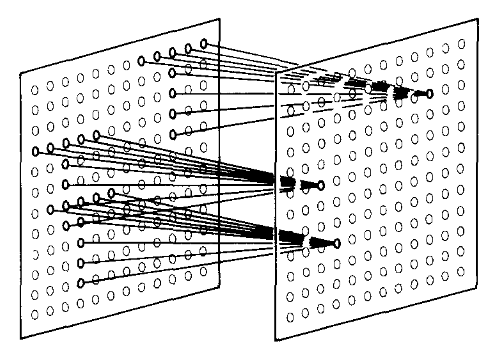
\includegraphics[width=0.3\linewidth]{images/3_receptive_field}
 \caption[Lokales rezeptives Feld]{Lokales rezeptives Feld (siehe \cite{Fukushima1980})}
 \label{fig:3_receptive_field}
 \end{figure}

Das \textit{LeNet} von \cite{LeCun1989} ist die Weiterentwicklung dieses Models. Hier teilen sich mehrere rezeptive Felder dieselben Gewichte beziehungsweise Parameter (\textit{Parameter Sharing}), was die Verbindungen und dadurch auch die Anzahl der Gewichte reduziert. Die Anzahl ist damit von der Dimensionalität der Eingabe entkoppelt. Algebraisch entspricht dies einer Faltung (\textit{Convolution}), wovon das Model seinen Namen ableitet. Diese Architektur ist die Grundlage heutiger CNNs und definiert die damit verbundenen Eigenschaften (vgl. \cite{LeCun1998}, \cite{Bengio2007b} und \cite{Zeiler2014}):
\begin{itemize}
\item Lokale Extraktion von Merkmalen (\textit{Local Feature Extraction})
\item Translationsinvarianz hinsichtlich Eingabedaten (geringe Skalierungs- und Rotationsinvarianz)
\item Einfacheres Training durch weniger Parameter und Verbindungen als MLP mit gleich vielen Neuronen
\item Nicht-lokale Generalisierung durch Verschachtlung nichtlinearer Funktionen
\end{itemize}

Abbildung \ref{fig:3_cnn} stellt ein CNN mit 8 Schichten zur Klassifikation von $32 \times 32$ Pixel großen Eingabebildern dar. Die ersten 6 Schichten zählen zum CNN, während die letzten beiden Schichten ein klassisches MLP repräsentieren. Der zugrundeliegende Ansatz ist hierbei, mittels CNN Merkmale (\textit{Features}) derart zu extrahieren, sodass die Klassen am Ende möglichst gut trennbar sind. 

\begin{figure}[H]
\centering
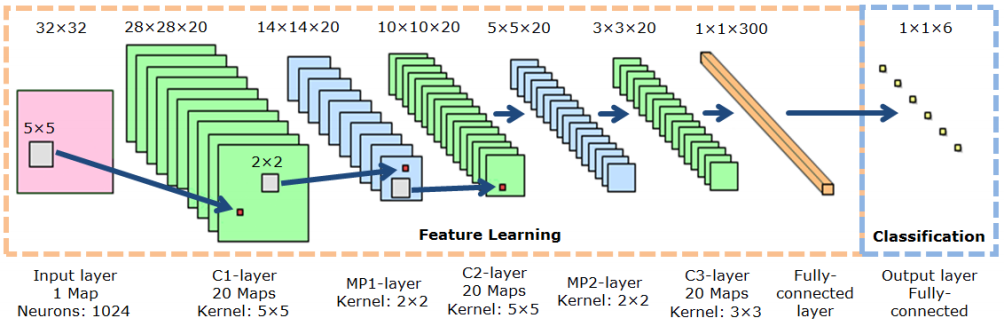
\includegraphics[width=0.95\linewidth]{images/3_CNN_Architecture}
\caption[Convolutional Neural Network mit 8 Schichten]{Convolutional Neural Network mit 8 Schichten \cite[siehe][]{Nagi2011}}
\label{fig:3_cnn}
\end{figure}

Aus Gründen der Vereinfachung werden im weiteren Verlauf des Kapitels lediglich quadratische Eingaben sowie quadratische Filtermasken betrachtet.

\subsubsection{Convolution-Layer}
Der Convolution-Layer ist einer der beiden zentralen Bestandteile eines CNN \cite[vgl. hierzu und im Folgenden][]{LeCun1998}. 
Dieser transformiert eine 3D-Eingabe $x$ mit Tiefe $m$, bezeichnet als $m$-\textit{Input-Maps}, zu einer 3D-Ausgabe $a$. Die Tiefe $n$ der Ausgabe wird bestimmt durch die Anzahl an Faltungskernen und selbst meist als $n$-\textit{Feature-Maps} bezeichnet. Ein Faltungskern $i$ ist in Abbildung \ref{fig:3_cnn_kernel} dargestellt. Er entspricht ebenfalls einer 3D-Struktur, welche durch Höhe $k_h$ und Breite $k_w$ der Faltungsmaske sowie der Tiefe $k_d$ bestimmt ist. Die Tiefe $k_d$ muss der Tiefe der 3D-Eingabe $m$ entsprechen. Es gibt somit gleich viele Faltungsmasken pro \textit{Feature-Map} wie es \textit{Input-Maps} gibt: Es gilt $k_d=m$. Alle Faltungskerne zusammen werden kompakt mit $W$ bezeichnet und einzelne Filtermasken mit $W_{ij}$ eindeutig indiziert.
Wird nun die Netz-Ausgabe (\textit{Forward Pass}) für eine \textit{Feature-Map} $i$ berechnet, muss für jede \textit{Input-Map} $x_j$ die Filtermaske $W_{ij}$ aus dem aktuellen Faltungskern gezogen und die Ausgabe $z_{ij}$ berechnet werden. Dies geschieht mittels diskreter Faltung. Die einzelnen Ausgaben $z_{ij}$ werden über alle \textit{Input-Maps} $1..m$ zu $z_i$ aufsummiert.

Die 3D-Ausgabe $a$ kann auch als Neuronen-Ausgabe interpretiert werden, in welcher jedes Element der Aktivierung eines Neurons entspricht. Bei der Berechnung eines $a_i$ wird folglich zu $z_i$ zunächst ein \textit{Bias} $b_i$ addiert und anschließend die Aktivierungsfunktion $\phi(\cdot)$ berechnet. Dies geschieht elementweise und analog für jede der $n$ \textit{Feature-Maps}.

\begin{figure}[H]
\centering
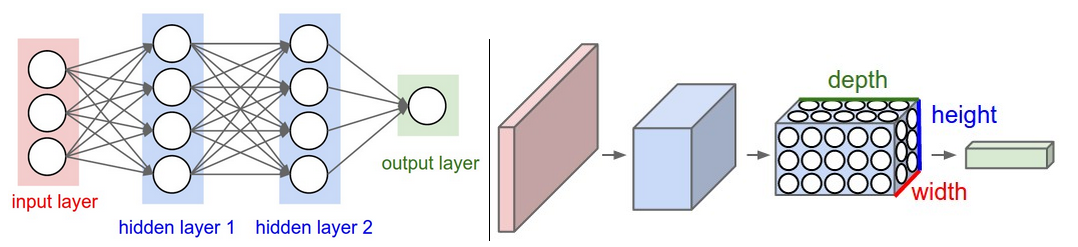
\includegraphics[width=0.95\linewidth]{images/3_cnn_kernel}
\caption[Jeder Convolution-Layer transformiert eine 3D-Eingabe (z.B. RGB-Bild) in eine 3D-Ausgabe]{Jeder Convolution-Layer transformiert eine 3D-Eingabe (z.B. RGB-Bild) in eine 3D-Ausgabe (siehe \cite{Kaparthy2014})}
\label{fig:3_cnn_kernel}
\end{figure}

Folgende Hyperparameter definieren einen Convolution-Layer:
\begin{itemize}
\item \textit{Feature-Maps}: $n$
\item \textit{Input-Maps}: $m = k_d$
\item Größe Faltungskern: $k_w = k_h$
\end{itemize}


Formal berechnet der Convolution-Layer für jede der $n$ \textit{Feature-Maps} zuerst die 2D-Faltung (Faltungsoperator: $\ast$) der $N \times N$-großen $m$ \textit{Input-Maps} mit der Filtermaske $W_{ij}$ (Gleichung \ref{eq:conv}) und im Anschluss elementweise die Aktivierungsfunktion $\phi(\cdot)$. Das Resultat ist die \textit{Feature-Map} $a_i$ (Gleichung \ref{eq:conv2}).
\begin{equation}
\label{eq:conv} 
z_i = \sum_{j=0}^{m}  x_{j} \ast W_{ij}
\end{equation}

\begin{equation}
\label{eq:conv2} 
a_{i} = \phi(z_{i} + b_i)
\end{equation}

Durch die Randbehandlung \textit{valid} reduziert sich die Größe der \textit{Feature-Maps} auf $(N - k_w + 1) \times (N - k_w + 1)$.\footnote{Es existieren bei der Faltung mehrere Modi zur Randbehandlung. Modus \textit{valid} berechnet nur die tatsächlich vorhandenen Elemente, wodurch die Ausgabe in der Größe schrumpft. Im Unterschied dazu berechnet der Modus \textit{full} die Faltung über eine mit Padding versehene Eingabe, wodurch sich die Ausgabe entsprechend vergrößert. Der Modus \textit{same} erzeugt eine gleich große Ausgabe.}

Die Anzahl der Gewichte berechnet sich aus $ n \cdot k_d \cdot k_w \cdot k_w$. Die Anzahl Pixel in der 3D-Ausgabe entspricht der Menge an Neuronen. Im Rahmen des Trainings gilt es, diese Gewichte zu trainieren. Die exakte mathematische Berechnung von Delta  $\delta$ und den partiellen Ableitungen $\frac{\partial J(W,b;x,y)}{\partial W_{ij}^l}$ und $\frac{\partial J(W,b;x,y)}{\partial b_i^l}$ für das Training mit Backpropagation folgt in Kapitel \ref{ch:cnn_back}.

\subsubsection{Pooling-Layer}
Der zweite wichtige Bestandteil eines CNN ist das sogenannte \textit{Pooling}. \cite{LeCun1998} bezeichnen diesen Vorgang als \textit{Subsampling}, wobei heute der Begriff \textit{Pooling} eher geläufig ist (vgl. \cite{Zeiler2013b} oder \cite{Glorot2011}).
Allgemein berechnet der Pooling-Layer ein Downsampling, wobei dessen Art nicht fest definiert ist. Abbildung \ref{fig:3_cnn_subsampling} stellt das sogenannte Max-Pooling dar (vgl. \cite{Glorot2011} und \cite{Zeiler2011}). 
Jede der $m$ \textit{Input-Map} $x_j$ der 3D-Eingabe wird vom Pooling-Layer einzeln bearbeitet und ausgegeben. Die Anzahl $m$ ändert sich nicht und es werden folglich $m$ \textit{Feature-Maps} erzeugt.
Für jedes $x_j$ wird nun ein Bereich der Größe $k_h \times k_w$, wobei $k_h$ der Filterhöhe und $k_w$ der Filterbreite entspricht, ausgeschnitten und verarbeitet. Im Falle des Max-Pooling wird das Maximum berechnet und in der Ausgabe gespeichert.

\begin{figure}[H]
\centering
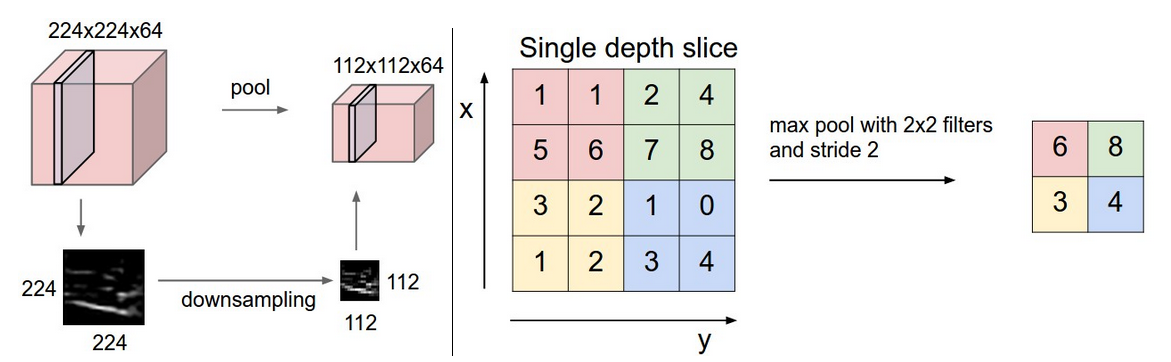
\includegraphics[width=0.95\linewidth]{images/3_cnn_subsampling}
\caption[Ein Pooling-Layer transformiert eine 3D-Eingabe (z.B. RGB-Bild) in eine kleinere 3D-Ausgabe (Downsampling)]{Ein Pooling-Layer transformiert eine 3D-Eingabe (z.B. RGB-Bild) in eine kleinere 3D-Ausgabe (Downsampling) (siehe \cite{Kaparthy2014})}.
\label{fig:3_cnn_subsampling}
\end{figure}

Folgende Hyperparameter sind damit für einen Pooling-Layer notwendig:
\begin{itemize}
\item Pooling-Methode
\item Filtergröße: $k_w = k_h$
\end{itemize}

Formal teilt der Max-Pooling-Layer jede \textit{Input-Map} $x_j$ in $k_w \times k_w$ disjunkte Bereiche und wählt in jedem Bereich das Maximum.
Dadurch reduziert sich die Ausgabe auf $ \frac{N}{k_w} \times \frac{N}{k_w}$.

Alternative, ebenfalls verbreitete Formen von Pooling stellen das \textit{Average}-Pooling \cite[vgl.][]{LeCun1998} oder das \textit{Lp}-Pooling \cite[vgl.][]{Sermanet2012} dar. 
Die Besonderheit beim Pooling-Layer sind die fehlende Aktivierungsfunktion sowie Gewichte und Schwellwerte, weshalb Convolution- und Pooling-Layer auch zusammen in einer Schicht berechnet werden können \cite[vgl.][]{Simard2003}.
Die exakte mathematische Beschreibung von Delta $\delta$ für das Training mit Backpropagation folgt in Kapitel \ref{ch:cnn_back}.

\subsection{Training mit Backpropagation}
\label{ch:cnn_back}
Im letzten Teil des Kapitels wurde bereits das Modell eines CNN und dessen elementaren Bestandteile beschrieben. Außerdem wurden die enthaltenen Parameter vorgestellt. Das Ziel dieses Abschnitts ist es zu beschreiben, wie die beiden neuen Schichten mittels Backpropagation trainiert werden können \cite[vgl. z.B.][]{Bouvrie2006}. Wie in Kapitel \ref{ch:backprop} beschrieben, ist für Backpropagation (Backward Pass) pro Trainingsbeispiel die Berechnung dreier Größen notwendig: $\delta^l$ sowie $\frac{\partial J(W,b;x_i,y_i)}{\partial W_{ij}^l}$ und $\frac{\partial J(W,b;x_i,y_i)}{\partial b_i^l}$. 

Um die Formeln zu vereinfachen, werden an dieser Stelle sogenannte \textit{Messages} eingeführt. Dies erleichtert die Notation insofern, dass die Berechnung von $\delta^l$ nicht mehr von den Gewichten der vorherigen Schicht $W^{l+1}$ abhängt. Delta $\delta_{message}^{l}$ bezeichnet so den über die Schicht hinaus zurück propagierten Fehler. Im Falle von gewöhnlichen MLPs gilt $\delta_{message}^{l+1} = (W^{l+1})^T\delta^{l+1}$. 
Für Convolutional-Layer wird das Delta $\delta_{i}^{l}$ korrespondierend zu jeder einzelnen der $n$-\textit{Feature-Maps} aus dem eingehenden $\delta_{message_j}^{l+1}$ berechnet. An dieser Stelle sei nochmals betont, dass die Anzahl \textit{Feature-Maps} $n$ der Anzahl \textit{Input-Maps} $m$ der nächsten Schicht entspricht. Es gilt folglich $n^l = m^{l+1}$. 
Im Folgenden werden zuerst die notwendigen Formeln für Pooling-Layer und im Anschluss die der Convolution-Layer vorgestellt.

Formel \ref{eq:convbackprop1} berechnet das Delta $\delta_{message_j}^{l}$ im Pooling-Layer mittels Kronecker-Produkt $kron(\cdot)$. Da der Pooling-Layer keine Parameter besitzt ist die Berechnung von $\delta_i^{l}$ irrelevant.

Delta Average-Pooling-Layer: \\
\begin{equation}
\label{eq:convbackprop1} 
\delta_{message_j}^{l} = kron(delta_{message_j}^{l+1}, ones(k_w,k_w)) \circ \frac{1}{k_w^2} 
\end{equation}

Je nach Pooling-Art muss hier unterschiedlich vorgegangen werden. Für einen Max-Pooling-Layer müssen im \textit{Forward Pass} die Positionen der Maxima gespeichert und bei der Rückpropagierung (Backward Pass) der Fehler an die gespeicherten Positionen geschrieben werden. Im Lp-Pooling muss der Fehler entsprechend der Norm $p$ und der verwendeten Filtermaske aufgeteilt werden.\\

Delta Convolution-Layer: \\
Für jede \textit{Feature-Map} $i$ im Convolution-Layer wird das zugehörige Delta $\delta_i^{l}$ mit Formel \ref{eq:convbackprop2a} berechnet. 
\begin{equation}
\label{eq:convbackprop2a} 
\delta_{i}^{l} =  \delta_{message_j}^{l+1} \circ \phi'(z_{i})
\end{equation}

Jedes $\delta_{message_j}^{l}$ für die Rückpropagierung des Fehlers wird mit Formel \ref{eq:convbackprop2b} berechnet.
Die Funktion $rot180(\cdot)$ bezeichnet das Drehen einer Matrix um $180^\circ$ beziehungsweise das Vertauschen beider Axen (\textit{Flipping}).
\begin{equation}
\label{eq:convbackprop2b} 
\delta_{message_j}^{l} = \sum_{i=0}^{n} \delta_{i}^{l} \ast rot180(W_{ij})
\end{equation}

Durch die Randbehandlung \textit{full} erhöht sich die Größe des Delta $\delta_{message_j}^l$ von $(N - k_w + 1) \times (N - k_w + 1)$ wieder auf  $N \times N$. \\


Gradient Convolution-Layer: \\
Der Gradient für den Convolution-Layer kann mittels Formel \ref{eq:convbackprop3} und \ref{eq:convbackprop4} aus der Eingabe $x$ und Delta $\delta^l$ berechnet werden. Die Randbehandlung \textit{valid} ist anzuwenden.
\begin{equation}
\label{eq:convbackprop3} 
\frac{\partial J(W,b)}{\partial W_{ij}^l} = \frac{1}{N} \sum_{e=1}^{N} rot180(x_{ej}^l \ast rot180(\delta_{ei}^l))                             
\end{equation}

\begin{equation}
\label{eq:convbackprop4}  
\frac{\partial J(W,b)}{\partial b_i^l} = \frac{1}{N} \sum_{e=1}^{N} \sum_{u=0}^{k_w} \sum_{v=0}^{k_w} \delta_{eiuv}^{l} 
\end{equation}

Analog zum Vorgehen bei MLPs wird der Gradient (Gleichung \ref{eq:convbackprop3} und \ref{eq:convbackprop4}) ebenfalls über alle Trainingsbeispiele $1..N$ aufsummiert und am Ende eines Durchlaufs mit $\frac{1}{N}$ gemittelt. Außerdem kann bei Aktivierungsfunktionen, deren Ableitung sich durch den Funktionswert selbst darstellen lässt, auf die Speicherung von $z$ verzichtet werden.

